
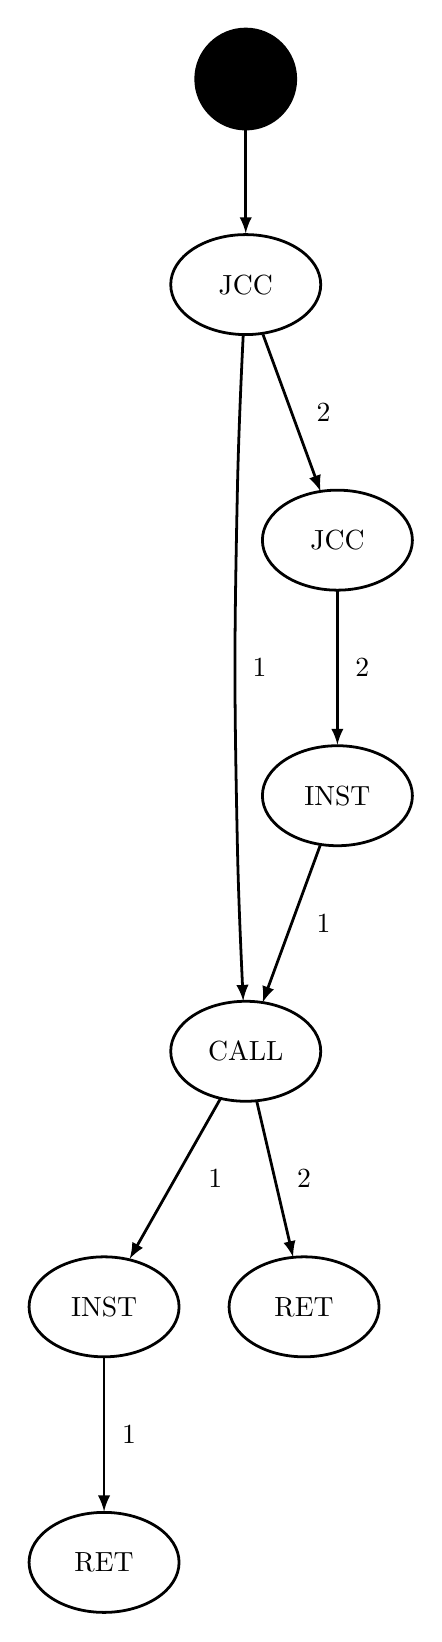
\begin{tikzpicture}[>=latex,line join=bevel,]
  \pgfsetlinewidth{1bp}
%%
\pgfsetcolor{black}
  % Edge: 2 -> 3
  \draw [->] (68.882bp,184.91bp) .. controls (61.242bp,171.43bp) and (50.2bp,151.94bp)  .. (36.211bp,127.25bp);
  \definecolor{strokecol}{rgb}{0.0,0.0,0.0};
  \pgfsetstrokecolor{strokecol}
  \draw (67.0bp,156.0bp) node {1};
  % Edge: 6 -> 7
  \draw [->] (111.0bp,367.65bp) .. controls (111.0bp,354.82bp) and (111.0bp,337.11bp)  .. (111.0bp,312.3bp);
  \draw (120.0bp,340.0bp) node {2};
  % Edge: 1 -> 6
  \draw [->] (84.207bp,460.07bp) .. controls (89.031bp,446.92bp) and (95.809bp,428.43bp)  .. (104.93bp,403.55bp);
  \draw (106.0bp,432.0bp) node {2};
  % Edge: 7 -> 2
  \draw [->] (104.79bp,276.07bp) .. controls (99.969bp,262.92bp) and (93.191bp,244.43bp)  .. (84.068bp,219.55bp);
  \draw (106.0bp,248.0bp) node {1};
  % Edge: 1 -> 2
  \draw [->] (77.098bp,459.9bp) .. controls (76.366bp,445.11bp) and (75.393bp,423.15bp)  .. (75.0bp,404.0bp) .. controls (73.832bp,347.12bp) and (73.832bp,332.88bp)  .. (75.0bp,276.0bp) .. controls (75.31bp,260.89bp) and (75.982bp,244.03bp)  .. (77.098bp,220.1bp);
  \draw (83.0bp,340.0bp) node {1};
  % Edge: 0 -> 1
  \draw [->] (78.0bp,533.94bp) .. controls (78.0bp,525.81bp) and (78.0bp,515.88bp)  .. (78.0bp,496.44bp);
  % Edge: 2 -> 5
  \draw [->] (81.95bp,184.07bp) .. controls (85.0bp,171.0bp) and (89.279bp,152.66bp)  .. (95.068bp,127.85bp);
  \draw (99.0bp,156.0bp) node {2};
  % Edge: 3 -> 4
  \draw [->] (27.0bp,91.647bp) .. controls (27.0bp,78.823bp) and (27.0bp,61.108bp)  .. (27.0bp,36.3bp);
  \draw (36.0bp,64.0bp) node {1};
  % Node: 1
\begin{scope}
  \definecolor{strokecol}{rgb}{0.0,0.0,0.0};
  \pgfsetstrokecolor{strokecol}
  \draw (78.0bp,478.0bp) ellipse (27.0bp and 18.0bp);
  \draw (78.0bp,478.0bp) node {JCC};
\end{scope}
  % Node: 0
\begin{scope}
  \definecolor{strokecol}{rgb}{0.0,0.0,0.0};
  \pgfsetstrokecolor{strokecol}
  \definecolor{fillcol}{rgb}{0.0,0.0,0.0};
  \pgfsetfillcolor{fillcol}
  \filldraw [opacity=1] (78.0bp,552.0bp) ellipse (18.0bp and 18.0bp);
\end{scope}
  % Node: 3
\begin{scope}
  \definecolor{strokecol}{rgb}{0.0,0.0,0.0};
  \pgfsetstrokecolor{strokecol}
  \draw (27.0bp,110.0bp) ellipse (27.0bp and 18.0bp);
  \draw (27.0bp,110.0bp) node {INST};
\end{scope}
  % Node: 2
\begin{scope}
  \definecolor{strokecol}{rgb}{0.0,0.0,0.0};
  \pgfsetstrokecolor{strokecol}
  \draw (78.0bp,202.0bp) ellipse (27.0bp and 18.0bp);
  \draw (78.0bp,202.0bp) node {CALL};
\end{scope}
  % Node: 5
\begin{scope}
  \definecolor{strokecol}{rgb}{0.0,0.0,0.0};
  \pgfsetstrokecolor{strokecol}
  \draw (99.0bp,110.0bp) ellipse (27.0bp and 18.0bp);
  \draw (99.0bp,110.0bp) node {RET};
\end{scope}
  % Node: 4
\begin{scope}
  \definecolor{strokecol}{rgb}{0.0,0.0,0.0};
  \pgfsetstrokecolor{strokecol}
  \draw (27.0bp,18.0bp) ellipse (27.0bp and 18.0bp);
  \draw (27.0bp,18.0bp) node {RET};
\end{scope}
  % Node: 7
\begin{scope}
  \definecolor{strokecol}{rgb}{0.0,0.0,0.0};
  \pgfsetstrokecolor{strokecol}
  \draw (111.0bp,294.0bp) ellipse (27.0bp and 18.0bp);
  \draw (111.0bp,294.0bp) node {INST};
\end{scope}
  % Node: 6
\begin{scope}
  \definecolor{strokecol}{rgb}{0.0,0.0,0.0};
  \pgfsetstrokecolor{strokecol}
  \draw (111.0bp,386.0bp) ellipse (27.0bp and 18.0bp);
  \draw (111.0bp,386.0bp) node {JCC};
\end{scope}
%
\end{tikzpicture}

